%%%%%%%%%%%%%%%%%%%%%%%%%%%%%%%%%

\section{Whitebox \& Blackbox Testing}

%%%%%%%%%%%%%%%%%%%%%%%%%%%%%%%%%

\begin{frame}
  \begin{center}
  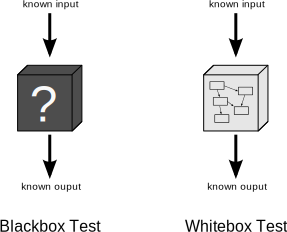
\includegraphics[width=.5\textwidth]{images/Qualitaetssicherung/abbildungen/BlackBoxAndWhiteBoxTesting}
  \end{center}
\end{frame}

%%%%%%%%%%%%%%%%%%%%%%%%%%%%%%%%%

\subsection{Whitebox Testing}

%%%%%%%%%%%%%%%%%%%%%%%%%%%%%%%%%
\begin{frame}
\frametitle{Whitebox Testing of Modules}
\framesubtitle{testing in the small}
\begin{description}[Anwei]
  \item[Statement Coverage:] \hfill \textbf{Statement coverage criterion}
  \begin{itemize}
    \item [] \small All executable statements in the source code are executed at least once.
  \end{itemize}
  \item[Edge coverage:] \hfill \textbf{Edge-coverage criterion}
  \begin{itemize}
    \item [] \small Each edge of the control graph being traversed at least once.
  \end{itemize}
  \item[Path (Branch) Coverage:] \hfill \textbf{Path-coverage criterion}
  \begin{itemize}
    \item [] \small All paths leading from the initial to the final node of the control graph being traversed.
  \end{itemize}
  \item[(Compound) Condition Coverage:] \hfill \textbf{Condition coverage criterion}
  \begin{itemize}
    \item [] \small Each possible combination of conditions must be executed at least once.
  \end{itemize}
\end{description}
\end{frame}

%%%%%%%%%%%%%%%%%%%%%%%%%%%%%%%%%

\subsection{Blackbox Testing}

%%%%%%%%%%%%%%%%%%%%%%%%%%%%%%%%%
\begin{frame}
\frametitle{Blackbox Testing of modules}
\framesubtitle{testing in the large}
\begin{enumerate}[align=parleft]
  \item [Idea:] A part of a program is tested without knowledge of the internal implementation.
  \item [Problem:] How to define the test set? 
  \begin{itemize}
  \item [] Defining the test set can only rely on the specification.
  \item [] Formal specifications are then a prerequisite for the systematic generation of test sets.
  \end{itemize}
\end{enumerate}
\end{frame}

%%%%%%%%%%%%%%%%%%%%%%%%%%%%%%%%%

\begin{frame}
\frametitle{Blackbox Testing of modules (contd.)}

\begin{enumerate}[align=parleft]
  \item [Method:] Derive test cases from the program specification.
  \begin{itemize}
  \item [] Disregard program structure.
  \end{itemize}
  \item [Pro:] Comprehensive but low-redundancy testing of the specified functionality.
  \begin{itemize}
  \item [] The key factor is the functional coverage.
  \end{itemize}
  \item [Con:] Oversight of functionality.
\end{enumerate}
\begin{block}{Defining a test case:}
    \begin{itemize}
      \item Functional equivalence class formation (equivalence class partitioning)
      \item Boundary value analysis (BVA)
      \item Special value testing
    \end{itemize}
\end{block}
\end{frame}